%----------------------------------------------------------------------------------------
%	PACKAGES AND OTHER DOCUMENT CONFIGURATIONS
%----------------------------------------------------------------------------------------
\documentclass[twoside]{article}

\usepackage[sc]{mathpazo} % Use the Palatino font
\usepackage[english]{babel}
\usepackage[utf8]{inputenc}
\usepackage{lipsum}
\usepackage{graphicx}
%\usepackage[T1]{fontenc} % Use 8-bit encoding that has 256 glyphs
\linespread{1.15} % Line spacing - Palatino needs more space between lines
\usepackage{microtype} % Slightly tweak font spacing for aesthetics

\usepackage[hmarginratio=1:1,top=32mm,columnsep=20pt]{geometry} % Document margins
\usepackage{multicol} % Used for the two-column layout of the document
\usepackage[hang, small,labelfont=bf,up,textfont=it,up]{caption} % Custom captions under/above floats in tables or figures
\usepackage{mathtools}
\usepackage{booktabs} % Horizontal rules in tables
\usepackage{float} % Required for tables and figures in the multi-column environment - they need to be placed in specific locations with the [H] (e.g. \begin{table}[H])
\usepackage{hyperref} % For hyperlinks in the PDF
\usepackage{wrapfig}
%\usepackage[]{mcode} % For embebing matlab code
\usepackage[makeroom]{cancel}

%\usepackage{lettrine} % The lettrine is the first enlarged letter at the beginning of the text
\usepackage{paralist} % Used for the compactitem environment which makes bullet points with less space between them

\usepackage{datetime}
\newdateformat{monthyeardate}{\monthname[\THEMONTH], \THEYEAR}
%\newdateformat{today}{\monthname[\THEMONTH], \date \THEYEAR}

\usepackage{abstract} % Allows abstract customization
\renewcommand{\abstractnamefont}{\normalfont\bfseries} % Set the "Abstract" text to bold
\renewcommand{\abstracttextfont}{\normalfont\small\itshape} % Set the abstract itself to small italic text

\usepackage{titlesec} % Allows customization of titles
%\renewcommand\thesection{\Roman{section}} % Roman numerals for the sections
%\renewcommand\thesubsection{\Roman{subsection}} % Roman numerals for subsections
\titleformat{\section}[block]{\large\scshape\centering}{\thesection.}{1em}{} % Change the look of the section titles
\titleformat{\subsection}[block]{\large\centering}{\thesubsection.}{1em}{} % Change the look of the section titles

\usepackage{fancyhdr} % Headers and footers
\pagestyle{fancy} % All pages have headers and footers
\fancyhead{} % Blank out the default header
\fancyfoot{} % Blank out the default footer
\fancyhead[C]{Astronomy % based on TRACS 
\hspace{4pt} $\bullet$ \hspace{4pt} Pleiades
\hspace{4pt} $\bullet$ \hspace{4pt} \monthyeardate\today} % Custom header text
\fancyfoot[RO,LE]{\thepage} % Custom footer text

\usepackage{cite}

\DeclareGraphicsExtensions{.pdf,.png,.jpg} % Graphics type

%----------------------------------------------------------------------------------------
%	   TITLE SECTION
%----------------------------------------------------------------------------------------

\title{
	\vspace{-15mm}
	\fontsize{28pt}{10pt}
	\selectfont\textbf{Photoelectric Photometry of the Pleaides}% Article title
}

\author{
	\large
	\textsc{Jaime Díez González-Pardo}\\[4mm]%\thanks{A thank you or further information}\\[2mm] % Your name
	\fontsize{28pt}{10pt} University of Cantabria \\ % Your institution
	%\thanks{A thank you or further information}\\[2mm] % Your name
	\normalsize Astronomy \\ 
	%\normalsize{Compañera:} \textsc{Mónica Escobedo}\\%\normalsize \href{mailto:john@smith.com}{john@smith.com} % Your email address
	%\vspace{5mm}
}

\date{ \usdate\today }


%----------------------------------------------------------------------------------------
%      · DOCUMENT
%----------------------------------------------------------------------------------------

\begin{document}


	\maketitle % Insert title


	\thispagestyle{fancy} % All pages have headers and footers

%----------------------------------------------------------------------------------------
%	  ABSTRACT
%----------------------------------------------------------------------------------------

	\begin{abstract}

		\noindent% Dummy abstract text

		The distance to the Pleiades' star cluster has been determine muassuring the apparent magnitude (for blue and visual filters) by means of a photometer using the program CLEA, and obtaining a value of $D = 125 \pm 14 \textrm{ pc} = 406 \pm 47 \textrm{ ly}$. To this aim, the Hertzsprung-Russell (\textbf{H-R}) diagram for the Pleiades star cluster has been compared with the (\textbf{H-R}) diagram of known main sequence stars, observing also the main sequence of the Pleiades cluster.

	\end{abstract}

%----------------------------------------------------------------------------------------
%	  ARTICLE CONTENTS
%----------------------------------------------------------------------------------------

	\begin{multicols}{2} % Two-column layout throughout the main article text

		\section{Introduction} % Scope of the project = rad effects + minimization

			Stars are continuously emitting energy which could be express in terms of its luminosity ($L = \frac{\mathrm{d} E}{\mathrm{d} t}$) or its flux ($F = \frac{L}{area}$). The apparent magnitud $m$ of a certain star, at unknown distance, is express in therms of the ratio of its flux $F$ over a reference flux $F_*$ by the equation \ref{eq:apparentTheo}.

				\begin{equation}
					m = -2.5 log_{10} \left(\frac{F}{F_*} \right)
					\label{eq:apparentTheo}
				\end{equation}

			As well, the absolute magnitud $M$ is defined as the apparent magnitud of the star if it were at a distance of $10$ pc. By this way, the absolute magnitud relate the apparent magnitud to the distancefrom the earth to the star. this relation is called the distance modulus $m-M$.

				\begin{equation}
					m-M = 5 log_{10} (D_{(pc)})-5
				\end{equation}

			Distance modulus expression were $D$ is the distance to the star en parsec. from this equation, an expression for the distance $D$ in function of its apparent and absolute magnitude can be obtained.

				\begin{equation}
					D = 10^{\frac{m-M}{5} +1}
					\label{eq:distanceTheo}
				\end{equation}

			Due to both magnitudes give information about the flux of stars, and therefore its energy, it could be used to determine the state of the star. One of the ways used to represent it is the Hertzsprung-Russell (\textbf{H-R}) diagram.

			In a Hertzsprung-Russell (\textbf{H-R}) diagram the absolute magnitud $M$ of a certain star cluster are plot as function of the spectral type ("Color index") which are related with the temperature of the star. In those types of diagram is posiblle to observe some defined regions which indicate the state of the star. 

				\begin{figure}[H]
					\centering
					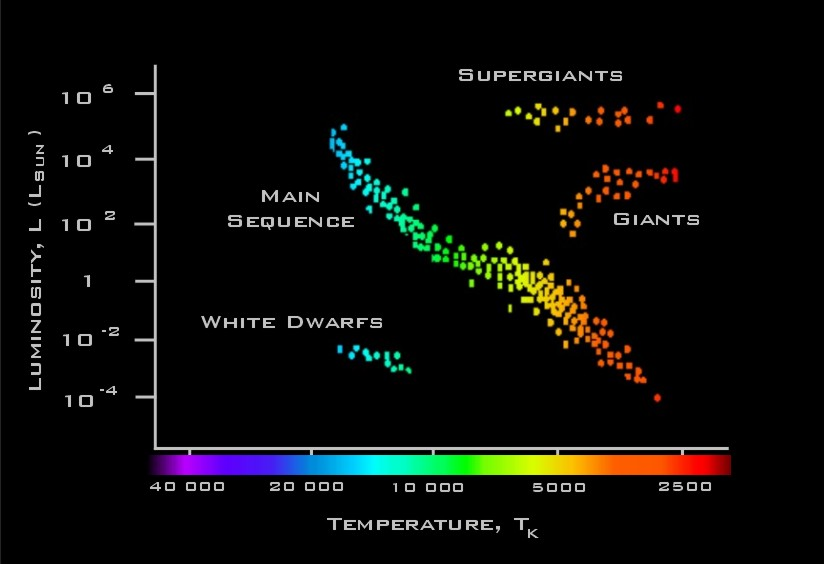
\includegraphics[scale=0.25]{Figures/hrcolour.jpg}
					\caption{\label{Img:HRTheo}Hertzsprung-Russell (\textbf{H-R}) diagram with four differents states of the stars: White Dwarfs, Main sequence, Giants and Super Giants. \cite{HRdiagram}}
				\end{figure}

			In Figure \ref{Img:HRTheo} an Hertzsprung-Russell (\textbf{H-R}) diagram is shown with four different regions corresponding to the evolutionary state of the star. The White Dwarf, in the left botton part of the diagram,the oldest with lowest luminosity but high temperature; Red Gigants and Supergigants, at top right; high luminosity and low temperature; and the Main sequence, the long diagonal line, where the stars spend most of their time.

		\section{Methods}

			In this experiment the CLEA program \textit{Photoelectric Photometry of the Pleiades} has been used to record the apparent magnitudes of 24 stars on the region of the Pleiades star cluster.

			This program allows to simulate the real procedure to take meassures in a real telescope, been necessary to request for bigger telescopes havin limit number of measuresfor each. For that reason meassures have been taken with three differents telescopes with diameters of 0.4, 1 and 4 meters.

			Once in the control panel, the corresponding star of study have been located by its coordinates archived in the program. The control panel allows to track the star in order to not lose it. This tracking is necessary due to, although the movement of the star is negligible form the earth, the earth is also rotating so the image of the star will move from east to west i opposite direction of the rotation move.

			Before measure the apparent magnitude of the star by the photometer is necessary to measure the background, by measure the sky, in order to minimaze the noise. This must be done for each filter in each telescope.

			After tracking the star and the sky noise has been measured, one of the posible filter ($B$, for blue, and $V$, for visual) has been selected and the measure started. The measure is made by means of integrations (number of times a measure is repeated) so it is necesary to select the wanted integrations and the duration of each integration. This selection is done trying to mantaing the signal noise, or $S/N$ ratio, in $100$. If this value is shown to increase or decrese, integrations or time should be change.

			Once the apparent magnitude in one of the filters is recorded, the filter is changed and the apparent magnitude measured again. Then, change the localization to another star and repeat the process.

		\section{Results}

			The apparent visual and blue magnitude ($m_V\textrm{ and }m_B$ respectivily) of 24 differents stars on the region of the Pleiades star cluster have been measured using the CLEA program \textit{Photoelectric Photometry of the Pleiades}. All the data obtained at the laboratory are shown in Table \ref{Tab:RawData}, in Appendix \ref{app:RawData}.

			In Figure \ref{Img:Apparent} the apparent visual magnitud, $m_V$, and the color index, $m_B - m_V$, are plotted in a Hertzsprung-Russell (\textbf{H-R}) diagram showing the main sequence of the stars.

				% Aparrent Magnitude
				\begin{figure}[H]
					\centering
					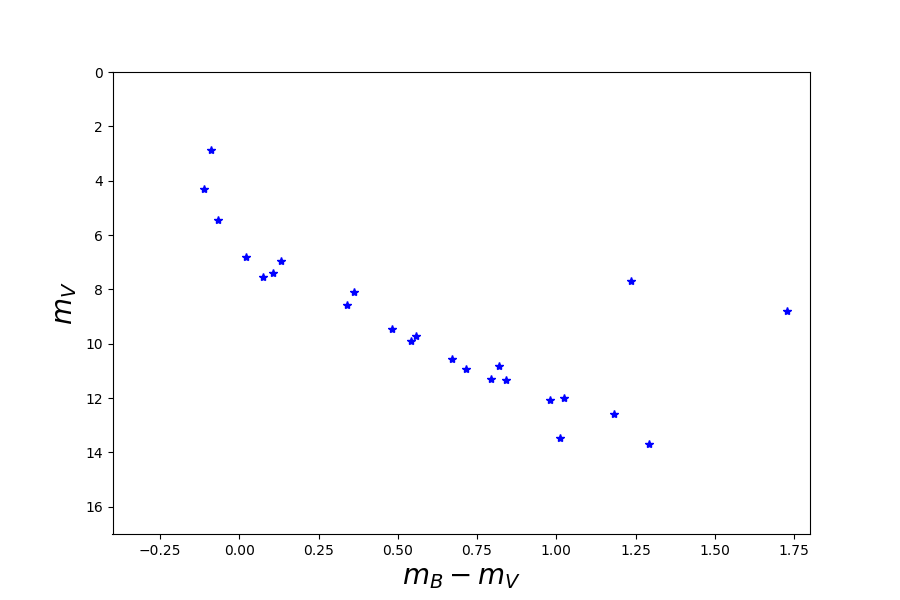
\includegraphics[scale=0.35]{Figures/expAparent.png}
					\caption{\label{Img:Apparent}(\textbf{H-R}) diagram of apparent visual magnitud $m_V$ of 24 differents stars on the region of the Pleiades star cluster as function of their color index $m_B - m_V$.}
				\end{figure}

			On the other hand, the absolute visual magnitude, $M_V$, of known main sequence stars, as well as the color index, $M_B - M_V$; are known \cite{Pleiades} and appear in Table \ref{Tab:GivenData}, in Appendix \ref{app:GivenData}.

			In Figure \ref{Img:Absolute} the absolute magnitude , $M_V$, and the color index, $M_B - M_V$, of the known main sequence stars \cite{Pleiades}, are plotted in a (\textbf{H-R}) diagram, showing again the main sequence of the stars.

				% Absolute Magnitude
				\begin{figure}[H]
					\centering
					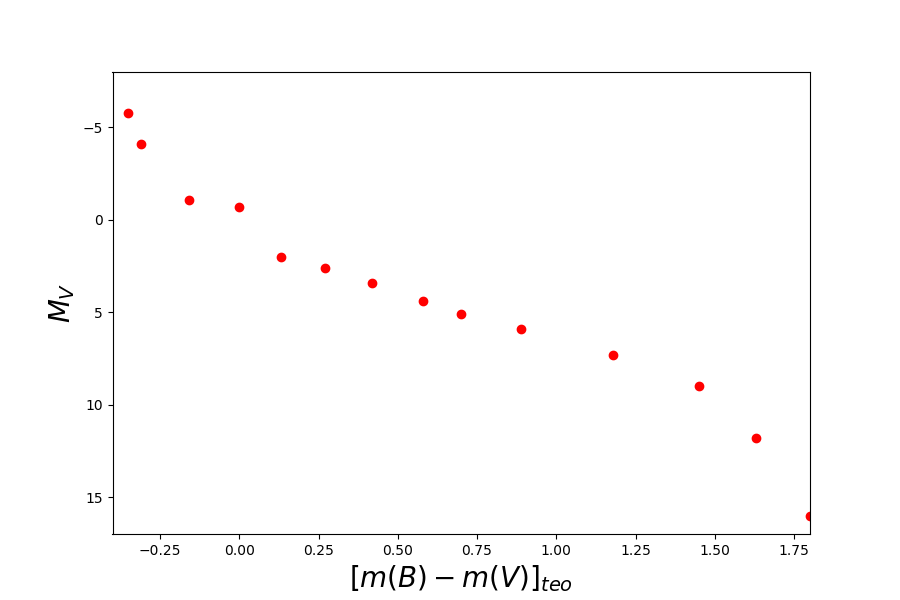
\includegraphics[scale=0.35]{Figures/theoabsolute.png}
					\caption{\label{Img:Absolute}(\textbf{H-R}) diagram of absolute visual magnitud $M_V$ of known main sequence stars as function of their color index $M_B - M_V$.}
				\end{figure}

			In order to compare both magnitudes, $M_V$ and $m_V$, they have been plotted in a same (\textbf{H-R}) diagram. However, due to some of the experimental values of the apparent visual magnitude $m_V$ at the edges of the diagram could be out the main sequence, only some values of both magnitudes at the $B-V$ \footnote{\label{ft:BV}$B$ and $V$ represent the corresponding magnitude for blue ($B$) or visual ($V$)} middle zone have been plotted.

			Table \ref{Tab:MiddleData} shows the values used in order to obtain the linear regression to determine the distance $D$.

				\begin{table}[H]
	\centering
	\begin{tabular}{ c  c || c  c }
		\\\hline
		\centering
			$M_B-M_V$ & $M_V$ & $m_B-m_V$ & $m_V$ \\\hline
			0.27 & 2.6 & 0.482 & 9.47 \\
			0.42 & 3.4 & 0.795 & 11.3 \\
			0.58 & 4.4 & 0.339 & 8.581 \\
			0.7 & 5.1 & 0.558 & 9.702 \\
			0.89 & 5.9 & 1.011 & 13.459 \\
			1.18 & 7.3 & 0.671 & 10.552 \\
			1.45 & 9.0 & 0.98 & 12.054 \\
			  &   & 1.025 & 12.007 \\
			  &   & 0.361 & 8.109 \\
			  &   & 0.541 & 9.897 \\
			  &   & 1.182 & 12.601 \\
			  &   & 1.291 & 13.689 \\
			  &   & 0.715 & 10.928 \\
			  &   & 0.818 & 10.821 \\
			  &   & 0.842 & 11.351 \\\hline
	\end{tabular}
	\caption{\label{Tab:MiddleData}Values at the $B-V$ middle zoneused to obtain the difference $m_V-M_V$. Two first columns corresponds to known main sequence stars. The other two columns corresponds to stars on the region of the Pleiades star cluster.}
\end{table}


			In Figure \ref{Img:Both} both visual apparent ($m_V$) and absolute ($M_V$) magnitudes have been plotted in a (\textbf{H-R}) diagram as a function of their color index ($B-V^{\ref{ft:BV}}$). Only stars at the the $B-V^{\ref{ft:BV}}$ middle zone are plotted.

				% Both
				\begin{figure}[H]
					\centering
					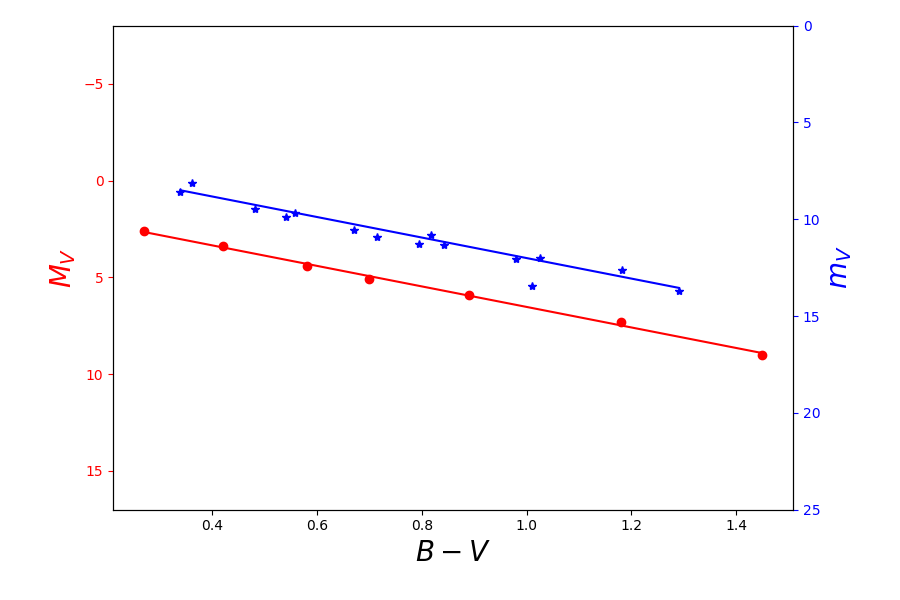
\includegraphics[scale=0.35]{Figures/both.png}
					\caption{\label{Img:Both}Visual apparent ($m_V$, blue stars) and absolute ($M_V$, red dots) magnitudes as a function of their color index ($B-V^{\ref{ft:BV}}$). Y-axis range are different for both magnitudes been $[17, -8]$ for $M_V$ and $[25, 0]$ for $m_V$. Both adjust have been done by a linear regression.}
				\end{figure}

			The linear regression done allow to obtain slopes and intercepts for both magnitudes. This values appear in Table \ref{Tab:Regression}.

				% Linear Regression values
				\begin{table}[H]
					\centering
					\begin{tabular}{c || c c}
						\hline
						\centering
							 & Slope & Intercept  \\ \hline
							$m_V$ & $5.3 \pm 0.3$ & $6.7 \pm 0.2$ \\ 
					        $M_V$ & $5.30 \pm 0.12$ & $1.23 \pm 0.11$ \\ \hline
					\end{tabular}
					\caption{\label{Tab:Regression}Slopes and intercepts for both magnitudes with their standard deviation [\ref{app:calc}].}
				\end{table}

			Both slopes are shown to be equal, which means both adjust are paralel each other. Thus the difference between both magnitudes' adjust must be the same for whatever color index value. The difference $m_V - M_V$ is going to be obtained by means of intercepts values which correspond to a star with color index $B - V = 0$.

				\begin{equation}
					m_V^{intercept} - M_V^{intercept} = 5.5 \pm 0.3 
				\end{equation}

			Once the difference has been determined, the distance $D$, in parsec, can be calculate by equation \ref{eq:distanceTheo}. The value of $D$ in light years has been obtained taking into account that $1 \textrm{ pc} = 3.26156 \textrm{ ly}$.

				\begin{equation}
					D = 125 \pm 14 \textrm{ pc} = 406 \pm 47 \textrm{ ly}
				\end{equation}

		\section{Conclussions}

			Three different telescopes with diameters of 0.4, 1 and 4 meters have been used in order to meassure the apparent magnitude of 24 stars on the region of the Pleiades star cluster by means of a photometer with two filters,  blue filter $m_B$ and visual filter $m_V$, been able to obtain their color index and, therefore, a (\textbf{H-R}) diagram.

			From that diagram, it has been possible to determine that almost all the stars measured are in the main sequence. There are two stars ($N2230-00985$ and $N2230-02192$) that differ above the main sequence coulding be two Red Giants according to the diagram of the Figure \ref{Img:HRTheo}. As well, the star $N2230-01554$ differs below the main sequence coulding be a White Dwarf. 

			The index color ($B-V$) of the (\textbf{H-R}) gives information about the range of emision of stars, and therefore, its temperature. The hottest star would emites in the blue range with the lowest color index ($B-V$) value. By this terms and according to the diagram \ref{Img:Apparent}, the hottest star meassured is $N2230-01585$ with an color index $B-v = -0.11$. On the other hand, the apparent visual magnitude $m_V$ is related by equation \ref{eq:apparentTheo} with the luminosity. Lower apparent magnitud means higher luminosity, so for stars of Table \ref{Tab:RawData} in the diagram \ref{Img:Apparent} the brightest star is $N2230-02202$.

			Once linear regression of both magnitudes in the (\textbf{H-R}) diagram have been done is possible to obtain the absolute or apparent magnitude for whatever star from its color index $B-V$ by the adjust equation given by the slope and the intercept. By this way, the absolute and apparent magnitud can be calculated for the Sun (type $G2$ and $B-V = 0.62$) if it were in the Pleiades cluster.

			Comparing those values with absolute magnitud of known main sequence stars, the distance to the Pleiades star cluster has been obtained with a final value of $D = 406 \pm 47 \textrm{ ly}$. This value is compatible and very similiar which the obtained in In 1958 by \textit{H.L. Johnson} and \textit{R.I. Mitchell} of $410 \textrm{ly}$. The discrepancy between both values is about less than $1\%$.

				\begin{equation}
					\begin{matrix}
						M_V = 5.30 \cdot (0.62) + 1.23 = 4.516
						\\
						\\
						m_V = 5.3 \cdot (0.62) + 6.7 = 9.986
					\end{matrix}
				\end{equation}



	\end{multicols}

%----------------------------------------------------------------------------------------
%     BIBLIOGRAPHY
%----------------------------------------------------------------------------------------

	\bibliographystyle{unsrt}
	\bibliography{../../biblio}

%----------------------------------------------------------------------------------------
%     APPENDIX
%----------------------------------------------------------------------------------------


			\appendix

				\section{Given Data of the Absolute Magnitud}
					\label{app:GivenData}

					\begin{table}[H]
	\centering
	\begin{tabular}{ c  c }
		\\\hline
		\centering
			$M_V$ & $M_B-M_V$ \\\hline
			-5.8 & -0.35 \\
			-4.1 & -0.31 \\
			-1.1 & -0.16 \\
			-0.7 & 0.0 \\
			2.0 & 0.13 \\
			2.6 & 0.27 \\
			3.4 & 0.42 \\
			4.4 & 0.58 \\
			5.1 & 0.7 \\
			5.9 & 0.89 \\
			7.3 & 1.18 \\
			9.0 & 1.45 \\
			11.8 & 1.63 \\
			16.0 & 1.8 \\\hline
	\end{tabular}
	\caption{\label{Tab:GivenData}Given values for visual absolute magnitude $M_V$ and color index $M_B-M_V$ of main sequence stars \cite{Pleiades}.}
\end{table}


			\newpage

				\section{Raw Data Obtained in the Laboratory}
					\label{app:RawData}

					\begin{table}[H]
	\centering
	\begin{tabular}{ c  c  c  c  c }
		\\\hline
		\centering
			Object-ID & RA & Dec & B & V \\\hline
			N2230-01442 & 3h41m18.0s & $23^o58'00"$ & 10.539 & 8.81 \\
			N2230-00478 & 3h42m55.1s & $24^o29'36"$ & 9.952 & 9.47 \\
			N2230-00526 & 3h44m06.6s & $24^o20'12"$ & 12.095 & 11.3 \\
			N2230-00306 & 3h45m06.5s & $24^o15'50"$ & 8.92 & 8.581 \\
			N2230-01585 & 3h45m12.5s & $24^o28'02"$ & 4.18 & 4.29 \\
			N2230-00156 & 3h45m40.2s & $24^o37'39"$ & 10.26 & 9.702 \\
			N2230-01554 & 3h45m42.4s & $25^o03'26"$ & 14.47 & 13.459 \\
			N2230-00319 & 3h45m43.2s & $24^o16'13"$ & 11.223 & 10.552 \\
			N2230-00990 & 3h45m48.4s & $24^o52'43"$ & 13.034 & 12.054 \\
			N2230-01908 & 3h46m27.3s & $24^o15'18"$ & 7.51 & 7.404 \\
			N2230-02089 & 3h46m27.8s & $23^o35'35"$ & 13.032 & 12.007 \\
			N2230-01621 & 3h46m34.2s & $23^o37'27"$ & 8.47 & 8.109 \\
			N2230-01627 & 3h46m50.5s & $23^o14'22"$ & 10.438 & 9.897 \\
			N2230-02081 & 3h46m59.3s & $24^o31'12"$ & 6.83 & 6.81 \\
			N2230-01820 & 3h47m01.4s & $24^o22'24"$ & 13.783 & 12.601 \\
			N2230-02202 & 3h47m29.1s & $24^o06'18"$ & 2.78 & 2.87 \\
			N2230-02192 & 3h47m36.9s & $23^o36'34"$ & 8.942 & 7.707 \\
			N2230-02091 & 3h47m50.8s & $24^o40'45"$ & 14.98 & 13.689 \\
			N2230-02449 & 3h48m13.4s & $25^o05'56"$ & 11.643 & 10.928 \\
			N2230-02207 & 3h48m20.8s & $23^o25'16"$ & 5.367 & 5.434 \\
			N2230-01601 & 3h48m30.1s & $24^o20'44"$ & 7.078 & 6.948 \\
			N2230-01175 & 3h49m07.5s & $24^o00'40"$ & 11.639 & 10.821 \\
			N2230-01127 & 3h49m25.1s & $23^o47'42"$ & 12.193 & 11.351 \\
			N2230-00985 & 3h49m56.6s & $24^o20'56"$ & 7.629 & 7.554 \\\hline
	\end{tabular}
	\caption{\label{Tab:RawData}Raw data obtained in the laboratory using the CLEA program Photoelectric Photometry of the Pleiades. Three first columns with the Id of each star ({\normalfont Object-ID}) and their coordenates ({\normalfont RA} and {\normalfont Dec}) are used in order to locate the star. The two last columns are the apparent magnitudes of each star meassured by the photometer with the blue filter {\normalfont B} and the visual filter {\normalfont V}.}
\end{table}


				\section{All The Calculus}
					\label{app:calc}

					All the calculus done in the report, including linear regressions, graphs, and errors propagation have been done using a script wrote by the student in python and available in \cite{github}.

\end{document}

%--------------------------------------------------------------------------------------
%            TEMPLATES
%--------------------------------------------------------------------------------------

%----------------------------------------------------------------------------------------
%            how to insert an image
%----------------------------------------------------------------------------------------

%	\begin{figure}[H]
%		\centering
%		\includegraphics[scale= ]{nombre de la imagen.jpg}
%		\caption{\label{Img:widgets}el pie de pagina que le quieras 	poner a la imagen}
%	\end{figure}
 
%----------------------------------------------------------------------------------------
%            how to insert a table
%----------------------------------------------------------------------------------------

%	\begin{table}[H]
%		\centering
%		\begin{tabular}{|c|c|c|c|}
%			\hline
%			\centering
%				Altura(h) & Distancia (d) & Elaboracion (e) & Longitud (l) \\
%				($\pm0.5$ mm) & ($\pm0.5$ mm) & ($\pm0.5$ mm) & ($\pm0.5$ mm) \\ \hline
%				 &  &  &  \\ \hline
%				 &  &  &  \\ \hline
%				 &  &  &  \\ \hline
%				 &  &  &  \\ \hline
%				 &  &  &  \\ \hline
%		         &  &  &  \\ \hline
%		\end{tabular}
%		\caption{\label{Tab:widgets}pie de pagina que le quieras poner}
%	\end{table}

%----------------------------------------------------------------------------------------
%             How to remove the label in equactions
%----------------------------------------------------------------------------------------

%	\begin{equation*}
%		
%	\end{equation*}

%----------------------------------------------------------------------------------------
%              How to set bibliography
%----------------------------------------------------------------------------------------

%\bibliographystyle{unsrt}
%\bibliography{biblio}
%
%Then you have to set a .bib document such as the next template
%
%	@book{nickname,
%	author = {},
%	title = {},
%	edition = {},
%	year = {},
%	volume = {},
%	ISBN = {}
%	}
%
%	@ARTICLE{nickname,
%	author = {},
%	title = {},
%	year = {},
%	volume = {},
%	}


%----------------------------------------------------------------------------------------
%              END
%----------------------------------------------------------------------------------------